\documentclass{article}
\usepackage{graphicx} % Required for inserting images
\usepackage[polish]{babel}
\usepackage{minted}
\usepackage[letterpaper,top=2cm,bottom=2cm,left=3cm,right=3cm,marginparwidth=1.75cm]{geometry}
\usepackage{amsmath}
\usepackage{graphicx}
\usepackage[colorlinks=true, allcolors=blue]{hyperref}
\usepackage[T1]{fontenc}
\usepackage[table,xcdraw]{xcolor}
\makeatletter
\renewcommand{\paragraph}{\@startsection{paragraph}{4}{0ex}%
   {-3.25ex plus -1ex minus -0.2ex}%
   {1.5ex plus 0.2ex}%
   {\normalfont\normalsize\bfseries}}
\makeatother

\stepcounter{secnumdepth}
\stepcounter{tocdepth}

\title{MOwNiT - Potównanie metod interpolacji i aproksymacji}
\author{Jakub Frączek}
\date{April 2024}

\begin{document}

\maketitle

\section{Funkcja dla której przeprowadzone zostało doświadczenie}

\begin{center}
\(f(x) = 10 * m + \frac{\mathrm{x}_{}^{2}}{k} - 10 * m * cos(k*x)\)
\end{center}

\noindent
gdzie:

\bigbreak

\(k = 1.5\)
\newline \indent
\(m = 3.0\)
\newline \indent
\(x \in [-4\pi, 4\pi]\)

\bigbreak

\noindent
Wykres funkcji:

\begin{figure}[H]
  \centering
  \begin{minipage}[b]{0.5\textwidth}
    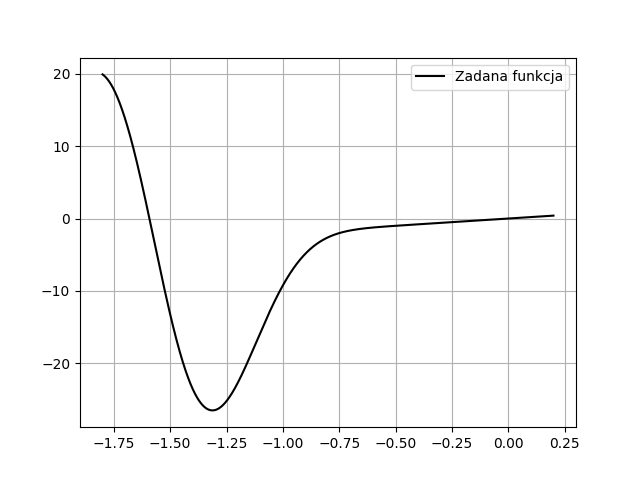
\includegraphics[width=\textwidth]{zadana_funkcja.png}
  \end{minipage}
\end{figure}

\section{Dane techniczne}

\subsection{Hardware}

Laptop z procesorem Intel Core i5-9300H 2.4GHz oraz 32 GB pamięci RAM.

\subsection{Software}

Wykorzystany został system Windows 11 x64 oraz język Python w wersji 3.11.8 wraz z bibliotekami:
\begin{itemize}
\item math
\item copy
\item matplotlib
\item numpy
\end{itemize}

\newpage

\section{Metody przyblizania funkcji}

\subsection{Interpolacja}

Jest to metoda, która polega na wyznaczeniu funkcji interpolującej, która w danym przedziale przyjmuje ustalone wartości w z góry zadanych punktach. Funkcja interpolująca może być wielomianem algebraicznym lub składać się z kilku funkcji.

\subsubsection{Interpolacja Lagrange'a}

Wielomian interpolacyjny Lagrange'a można wyrazić wzorem:
\[\sum_{k=0}^{n} f(\mathrm{x}_{k}^{})\mathrm{L}_{k}^{}\]
gdzie:
\bigbreak
\( f(\mathrm{x}_{k}^{})\ -\ wartości\ funkcji\ w\ punktach\ \mathrm{x}_{k}^{} \)
\bigbreak
\( \mathrm{L}_{k}^{}(x) = \frac{d}{m} = \prod_{i\ =\ 0, i\ !=\ k}^{n}\ \frac{x -\mathrm{x}_{i}^{}}{\mathrm{x}_{k}^{} - \mathrm{x}_{i}^{}}\ - \ baza\ Lagrange'a\)

\subsubsection{Interpolacja Newtona}

\[ \mathrm{P}_{n}^{}(x) = f[\mathrm{x}_{0}^{}] + \sum_{i = 1}^{n}f[\mathrm{x}_{0}^{}, \mathrm{x}_{1}^{}, ..., \mathrm{x}_{i}^{}]*(x - \mathrm{x}_{0}^{})*(x - \mathrm{x}_{1}^{})*...*(\mathrm{x}_{i - 1}^{})\]

\noindent
gdzie:
\bigbreak

\( f[\mathrm{x}_{i}^{}] = f(\mathrm{x}_{i}^{}) \) \newline \indent
\( f[\mathrm{x}_{i}^{}, \mathrm{x}_{i+1}^{}] = \frac{f[\mathrm{x}_{i+1}^{}]-f[\mathrm{x}_{i}^{}]}{\mathrm{x}_{i+1}^{}-\mathrm{x}_{i}^{}} \) \newline \indent
\( . \) \newline \indent
\( . \) \newline \indent
\( . \) \newline \indent
\( f[\mathrm{x}_{i}^{}, \mathrm{x}_{i+1}^{}, ..., \mathrm{x}_{i + k}^{}] =
\frac{f[\mathrm{x}_{i+1}^{}, \mathrm{x}_{i+2}^{}, ..., \mathrm{x}_{i + k}^{}] - f[\mathrm{x}_{i}^{}, \mathrm{x}_{i+1}^{}, ..., \mathrm{x}_{i + k -1}^{}]}{\mathrm{x}_{i+k}^{} - \mathrm{x}_{i}^{}} \) \newline

\subsubsection{Interpolacja Hermite'a}

\[\mathrm{H}_{n}^{}(x) = \sum_{i = 0}^{n}\mathrm{b}_{l}^{}\mathrm{p}_{l}^{}(x) = 
\sum_{i = 0}^{k}\sum_{j=0}^{\mathrm{m}_{i}^{} - 1}\mathrm{b}_{(s(i) + j)}^{} \cdot 
\mathrm{p}_{s(i) + j}^{}(x) \]

\noindent
gdzie:

\bigbreak

\(\mathrm{p}_{s(0)}^{}(x) = 1\) 

\indent

\(\mathrm{p}_{s(i) + j}^{}(x) = \mathrm{(\mathrm{x - \mathrm{x}_{0}^{}}_{}^{})}_{}^{\mathrm{m}_{0}^{}}
\mathrm{(\mathrm{x - \mathrm{x}_{1}^{}}_{}^{})}_{}^{\mathrm{m}_{1}^{}}...
\mathrm{(\mathrm{x - \mathrm{x}_{i - 1}^{}}_{}^{})}_{}^{\mathrm{m}_{i-1}^{}}
\mathrm{(\mathrm{x - \mathrm{x}_{i}^{}}_{}^{})}_{}^{\mathrm{j}_{}^{}}\)

\indent

\(
s(i) = 
\begin{cases}
    0 & \text{dla } i = 0 \\
    \mathrm{m}_{0}^{} + \mathrm{m}_{1}^{} + ... + \mathrm{m}_{i - 1}^{} & \text{dla } i > 0
\end{cases}
\)

\indent

\(i = 0, 1, ..., k\)

\indent

\(j = 0,1,...,\mathrm{m}_{i}^{} - 1\)

\indent

Współczynniki \(\mathrm{b}_{l}^{}\) to kolejne ilorazy różnicowe.

\newpage

\subsubsection{Kwadratowa funkcja sklejana}

\paragraph{Wyznaczanie współczynników}

Kwadratowa funkcja sklejona musi spełniać warunki:

\begin{itemize}
    \item \( S_i (x) = a_i + b_i(x - x_i) + c_i(x - x_i)^2\) \ (1)
    \item \(S_i(x_i) = f(x_i) = y_i\) (2)
    \item \(s_i(\mathrm{x}_{i+1}^{}) = S_{i + 1}(x_{i+1})\) \ (3)
    \item \(S'_i(x_{i+1}) = S'_{i+1}(x_{i+1})\) \ (4)
\end{itemize}

\noindent
Podstawiam \(x_i\) do (1) i korzystam z właności (2), z tego otrzymuję:

\[y_i = S_i (x_i) = a_i + b_i(x_i - x_i) + c_i(x_i - x_i)^2 = a_i \Rightarrow  a_i = y_i \ \ (5)\] 
\noindent
Korzystając z warunku (1) i (4):

\[b_{i+1} + 2c_{i+1}(x_{i+1}-x_{i+1}) = b_i + 2c_i(x_{i+1} - x_i)\]

\[b_{i+1} = b_i + 2c_i(x_{i+1} - x_i)\]

\[c_i = \frac{b_{i+1}-b_i}{2(x_{i+1}-x_i)} \ \ (6)\] 
\noindent
Korzystając z (1), (2), (3) i (5):

\[y_{i+1} = S_i(x_{i+1}) = S_{i+1}(x_{i+1}) = y_i + b_i(x_{i+1} - x_i) + c_i(x_{i+1}-x_i)^2 \ \ (7)\]
\noindent
Korzystając z (6) i (7):

\[y_{i+1} - y_i = b_i(x_{i+1}-x_i) + \frac{b_{i+1}-b_i}{2(x_{i+1}-x_i)}(x_{i+1}-x_i)^2\]

\[\frac{y_{i+1} - y_i}{x_{i+1}-x_i} = b_i + \frac{1}{2}b_{i+1} - \frac{1}{2}b_i\]

\[2\cdot \frac{y_{i+1} - y_i}{x_{i+1}-x_i} = b_{i+1}+b_i\]

\[b_i + b_{i-1} = 2\frac{y_i - y_{i-1}}{x_i - x_{i-1}}\]
\noindent
Oznaczam \(\frac{y_i - y_{i-1}}{x_i - x_{i-1}}\) jako \(v\) i tworzę układ równań w celu wyliczenia
wspołczynnika \(b_i\)

\bigbreak

\[b_1 + b_2 = 2v_2\]
\[b_2 + b_3 = 2v_3\]
\[\vdots\]
\[b_{n-2}+b_{n-1}=2v_{n-1}\]

\begin{gather*}
\begin{bmatrix}
1 & 1 & 0 & \cdots & 0 \\
0 & 1 & 1 & \ddots & \vdots \\
\vdots & \ddots & \ddots & \ddots & 0 \\
0 & \cdots & 0 & 1 & 1 
\end{bmatrix}  
\begin{bmatrix}
b_1 \\
b_2 \\
\vdots \\
b_{n-1} 
\end{bmatrix} 
=
\begin{bmatrix}
2v_1 \\
2v_2 \\
\vdots \\
2v_{n-1} 
\end{bmatrix}
\end{gather*}
\noindent
Jak widać jest n - 1 równań i n niewiadowmych, zatem trzeba będzie ustalić doddatkowy warunek brzegowy.

\paragraph{Natural Boundary}

Założenia:

\[S'_1(x_1) = 0 \ \ \vee \ \ S'_{n-1}(x_n) = 0 \ \ (8)\]
\noindent
Korzystając z (1) i (8):

\[S'_1(x_1) = 0 = b_1 + 2c_1(x_1-x_1) \Rightarrow b_1 = 0 \ \ (9)\]
\noindent
Zatem:

\[b_1+b_2 = 2v_2 \Rightarrow b_2 = 2v_2\]

\[b_2 + b_3 = 2v_3 \Rightarrow b_3 = 2v_3-2v_2\]

\[\vdots\]

\[b_n = 2(v_n-v_{n-1}+v_{n-2}-...\pm v_2)\]

\paragraph{Clamped Boundary}
\noindent
Założenia:

\[S'_1(x_1) = f'_1(x) \ \ \vee \ \ S'_{n-1}(x_n) = f'_{n-1}(x) \ \ (10)\]
\noindent
\(f'_1(x)\) można zapisać jako:
\[f'_1(x) = \frac{y_2-y_1}{x_2-x_1} \ \ (11)\]
\noindent
Korzystając z (1), (10) i (11):

\[b_1 + 2c_1(x_1 - x_1) = \frac{y_2 - y_1}{x_2-x_1} \Rightarrow  b_1 = \frac{y_2 - y_1}{x_2-x_1} = v_2\]

\bigbreak
\noindent
Zatem:

\[b_1 + b_2 = 2v_2 \Rightarrow b_2 = v_2\]

\[b_2 + b_3 = 2v_3 \Rightarrow b_3 = 2v_3 - v_2 \]

\[\vdots \]

\[b_n = 2(v_n-v_{n-1}+v_{n-2}+...\pm v_3) \pm v_2\]

\newpage

\subsubsection{Sześcienna funkcja sklejana}

\paragraph{Wyznaczanie współczynników}

Wzór na sześcienną funkcję sklejaną został podany poniżej:

\[s(x) = \mathrm{a}_{i}^{} + \mathrm{b}_{i}^{}\cdot (x - \mathrm{x}_{i}^{}) +\mathrm{c}_{i}^{}\cdot \mathrm{(x - \mathrm{x}_{i}^{})}_{}^{2} + \mathrm{d}_{i}^{}\cdot  \mathrm{(x-\mathrm{x}_{i}^{})}_{}^{3} \ dla \ x \in [\mathrm{x}_{i}^{}, \mathrm{x}_{i + 1}^{}]\]
\noindent
Dodatkowo funkcja sklejana 3-go stopnia musi spełniać poniższe warunki:
\begin{itemize}
\item \(S_i(x_{i+1}) = f(x_{i+1})\)
\item \(S_i(x_{i+1}) = S_{i+1}(x_{i+1})\)
\item \(S'i(x_{i+1}) = S'_{i+1}(x_{i+1})\)
\item \(S''(x_{i+1}) = S''_{i+1}(x_{i+1})\)
\end{itemize}
\noindent
Ponieważ \(S_i(x)\) jest sześcienna, to \(S''_i(x)\) jest liniowa na przedziale \([x_i, x_{i+1}]\). Wprowadzam \(h_i = x_{i+1} - x_i\), wtedy:

\[S''_i(x) = S''_i(x_i)\frac{x_{i+1}-x}{h_i} + s''_i(x_{i+1})\frac{x-x_i}{h_i}\]
\noindent
Całkując dwukrotnie otrzymuję:

\[S_i(x) = \frac{S''_i(x_i)}{6h_i}(x_{i+1}-x)^3 + \frac{S''_i(x_{i+1})}{6h_i}(x-x_i)^3+C(x-x_i)+D(x_{i+1}-x)\],
\noindent
gdzie C i D - stałe całkowania
\noindent
Korzystając z warunków interpolacji:
\noindent
\(S_i(x_i) = y_i\) oraz \(S_i(x_{i+1}) = y_{i+1}\) można wyliczyć C i D. Po wyliczeniu tych stałych otrzymujemy:

\[S_i(x) = \frac{S''_i(x_i)}{6h_i}(x_{i+1}-x)^3 + \frac{S''_i(x_{i+1})}{6h_i}(x-x_i)^3 + 
(\frac{y_{i+1}}{h_i} - \frac{S''_i(x_{i+1})h_i}{6})(x-x_i) + (\frac{y_i}{h_i}-\frac{S''_i(x_i)h_i}{6})(x_{i+1}-x)\]
\noindent
W powyższym wzorze nadal nie znamy \(S''_i(x)\). W celu jego wyliczenia należy skorzystać z warunku ciągłości pierwszech pochodnej. Różniczkuję zatem \(S_i(x)\):

\[S'_i(x_i) = -\frac{h_i}{3}S''_i(x_i) - \frac{h_i}{6}S''_i(x_{i+1}) - \frac{y_i}{h_i} + \frac{y_{i+1}}{h_i}\]
\noindent
Dla przejrzystości należy wprowadzić dwa symbole:
\begin{itemize}
\item \(\sigma_i = \frac{1}{6}S''(x_i)\)
\item \(\Delta_i = \frac{y_{i+1}-y_i}{h_i}\)
\end{itemize}
\noindent
Wtedy:

\[S'_i(x_i) = -2\sigma_ih_i - \sigma_{i+1}h_i + \Delta_i\]
\[S'_i(x_i) = \Delta_i - h_i(\sigma_{i+1}+2\sigma_i)\]
\noindent
Wtedy:

\[S'_{i-1}(x_i) = \Delta_{i-1} + h_{i-1}(2\sigma_i + \sigma_{i-1})\]
\noindent
Teraz korzystając z warunku ciągłości (\(S'_{i-1}(x_i) = S'_i(x_i)\)):

\[\Delta_{i-1} + h_{i-1}(2\sigma_i + \sigma_{i-1}) = \Delta_i - h_i(\sigma_{i+1} + 2\sigma_i)\]
\noindent
Finalnie otrzymujemy układ równań liniowych:

\[h_{i-1}\sigma_{i-1} + 2(h_{i-1}+h_i)\sigma_i + h_i\sigma_{i+1} = \Delta_i - \Delta_{i-1}, i = 2,3,...,n-1\]
\noindent
Jak można zauważyć w układzie równań mamy n niewiadomych i n - 2 równań, zatem należy określić dwa dodatkowe warunki brzegowe.

\paragraph{Default Boundary}

Warunki:

\begin{itemize}
\item \(C_1(x)\) - f. sześcienna przez pierwsze 4 punkty
\item \(C_n(x)\) - f. sześcienna przez ostatnie 4 punkty
\end{itemize}

\[S'''(x_1) = C'''_1 \ \ \ S'''(x_n) = C'''_n\]
\noindent
Stałe \(C'''_1 i C'''_n\) mogą być określone bez znajomości \(C_1(x)\) i \(C_n(x)\):

\begin{itemize}
\item \(\Delta_i^{(1)} = \frac{y_{i+1} - y_i}{x_{i+1}-x_i}\)
\item \(\Delta_i^{(2)} = \frac{\Delta_{i+1}^{(1)}-\Delta_i^{(1)}}{x_{i+2}-x_i}\)
\item \(\Delta_i^{(3)} = \frac{\Delta_{i+1}^{(2)}-\Delta_i^{(2)}}{x_{i+3}-x_i}\)
\end{itemize}
\noindent
Różniczkując wzór na \(S''(x)\) na przedziale \([x_i, x_{i+1}]\), otrzymujemy:

\[S'''(x_1) = C'''_1(x_1) \Rightarrow  \frac{6}{h_1}(\sigma_2-\sigma_1) = 6\Delta_i^{(3)}\]

\[S'''(x_n) = C'''_n(x_n) \Rightarrow  \frac{6}{h_{n-1}}(\sigma_n - \sigma_{n-1}) = 6\Delta_{n-3}^{(3)}\]
\noindent
Po przekształceniu otrzymujemy:

\begin{itemize}
\item \(-h_1\sigma_1 + h_1\sigma_2 = h_1^2\Delta_1^{(3)}\)
\item \(h_{n-1}\sigma_{n-1} - h_{n-1}\sigma_n = -h_{n-1}^2\Delta_{n-3}^{(3)}\)
\end{itemize}
\noindent
Finalnie otrzymujemy:

\begin{gather*}
\begin{bmatrix}
-h_1 & h_1 & 0 & 0 & 0 \\
h_1 & 2(h_1+h_2) & h_2 & 0 & 0 \\
0 & h_2 & 2(h_2+h_3) & h_3 & 0 \\
\vdots & \vdots & \vdots & \vdots & \vdots \\
0 & 0 & h_{n-2} & 2(h_{n-2} + h_{n-1}) & h_{n-1} \\
0 & 0 & 0 & h_{n-1} & -h_{n-1} 
\end{bmatrix}
\begin{bmatrix}
\sigma_1 \\
\sigma_2 \\
\sigma_3 \\
\vdots \\
\sigma_{n-1} \\
\sigma_n 
\end{bmatrix}
=
\begin{bmatrix}
\mathrm{h}_{1}^{2}\mathrm{\Delta}_{1}^{(3)} \\
\Delta_2 - \Delta_1 \\
\Delta_3 - \Delta_2 \\
\vdots \\
\mathrm{\Delta}_{n-1}^{} - \mathrm{\Delta}_{n-2}^{} \\
\mathrm{-h}_{n-1}^{2}\mathrm{\Delta}_{n-3}^{(3)} 
\end{bmatrix}
\end{gather*}

\paragraph{Natural Boundary}

Warunki:

\[S''(x_1) = S''(x_n) = 0\]
\noindent
Biorąc pod uwagę, że \(\sigma_i = \frac{1}{6}S''_i(x_i)\) otrzymujemy:

\[S''(x_1) = S''_1(x_1) = 0 \Leftrightarrow \sigma_1 = 0\]

\[S''(x_n) = S''_n(x_n) = 0 \Leftrightarrow \sigma_n = 0\]
\noindent
Dzięki temu otrzymujemy:

\begin{gather*}
\begin{bmatrix}
1 & 0 & 0 & 0 & 0 \\
h_1 & 2(h_1+h_2) & h_2 & 0 & 0 \\
0 & h_2 & 2(h_2+h_3) & h_3 & 0 \\
\vdots & \vdots & \vdots & \vdots & \vdots \\
0 & 0 & h_{n-2} & 2(h_{n-2} + h_{n-1}) & h_{n-1} \\
0 & 0 & 0 & 0 & 1 
\end{bmatrix}
\begin{bmatrix}
\sigma_1 \\
\sigma_2 \\
\sigma_3 \\
\vdots \\
\sigma_{n-1} \\
\sigma_n 
\end{bmatrix}
=
\begin{bmatrix}
0 
\Delta_2 - \Delta_1 \\
\Delta_3 - \Delta_2 \\
\vdots \\
\mathrm{\Delta}_{n-1}^{} - \mathrm{\Delta}_{n-2}^{} \\
0
\end{bmatrix}
\end{gather*}

\newpage

\subsection{Aproksymacja}

Polega na znalezieniu funkcji aproksymującej, która nie przechodzi przez wszystkie zadane punkty (tak jak było w interpolacji), tylko odzwierciedla ogólny trend w danych, tj. czasem przechodzi pomiędzy węzłami, tak by jak najlepiej dopasować się do funkcji.

\subsubsection{Aproksymacja średniokwadratowa wielomianami algebraicznymi}

\noindent
Funkcja bazowe, czyli ciągi jednomianów \(\varphi _j(x) = x^i, j = 0, 1, ..., m\)

\noindent
Funkcja aproksymująca: \(f(x) = \sum_{j=0}^{m}a_j\varphi_j(x) = \sum_{j=0}^{m}a_jx^i\)

\noindent
F(x) - zadana na zbiorze dyskretnym \(\{x_i\}, i = 0, 1, ..., n\)

\noindent
Szukamy takich współczynników \(a_j\), że:

\[min!\sum_{i=0}^{n}w(x_i)[F(x_i) - f(x_i)]^2\]

\noindent
Układ normalny:

\[\sum_{i = 0}^{n}w(x_i)[F(x_i) - \sum_{j=0}^{m}a_jx_i^j]x_i^{k\longleftarrow \frac{\partial f}{\partial a_k}} = 0, k = 0, 1, ..., m\]

\[\sum_{i = 0}^{n}w(x_i)x_i^k\sum_{j=0}^{m}a_jx_i^j = \sum_{i=0}^{n}w(x_i)F(x_i)x_i^k, k =0,1,...,m\]

\[\sum_{j=0}^{m}(\sum_{i=0}^{n}w(x_i)x_i^{j+k}a_j = \sum_{i=0}^{n}w(x_i)F(x_i)x_i^k\]

\noindent
W postaci macierzowej:

\begin{gather*}
\begin{pmatrix}
\Sigma w_i & \Sigma w_ix_i & \Sigma w_ix_i^2 & \cdots & \Sigma w_ix_i^m \\
\Sigma w_ix_i & \Sigma w_ix_i^2 & \Sigma w_ix_i^3 & \cdots & \Sigma w_ix_i^{m+1} \\
\vdots & \vdots & \vdots & \ddots & \vdots \\
\Sigma w_ix_i^m & \Sigma w_ix_i^{m+1} & \Sigma w_ix_i^{m+2} & \cdots & \Sigma w_ix_i^{2m} 
\end{pmatrix} 
\begin{pmatrix}
a_0 \\
a_1 \\
\vdots \\
a_m 
\end{pmatrix}
= 
\begin{pmatrix}
\Sigma w_iF_i \\
\Sigma w_iF_ix_i \\
\vdots \\
\Sigma w_iF_ix_i^m 
\end{pmatrix}
\end{gather*}

\[G \cdot A=B\]

\subsubsection{Aproksymacja średniokwadratowa wielomianami trygonometrycznymi}

Ogólny wzór na przybliżenie aproksymacyjne

\[F(x) = c_o\phi_o(x) + c_1\phi_1(x) + ... + c_m\phi_m(x) = \Sigma_{i=0}^{m}c_i\phi_i(x)\]

\noindent
W tym przypadku za funkcje bazowy przyjmuję
\[(\phi_i(x)) = 1, sin(x), cos(x), sin(2x), cos(2x), ..., sin(mx), cos(mx)\]

\noindent
Wzory przybliżające szukaną funkcję wielomianem trygonometrycznym

\[F_m(x) = \frac{1}{2} \cdot a_0 + \Sigma_{j=1}^{m}(a_j \cdot cos(j \cdot x) + b_j \cdot sin(j \cdot x)\]

\[a_j = \frac{2}{n} \cdot \Sigma_{i=0}^{n-1}f(x_i) \cdot cos(j \cdot x_i)\]

\[b_j = \frac{2}{n} \cdot \Sigma_{i=0}^{n-1}f(x_i) \cdot sin(j \cdot x_i)\]

\noindent
Przyjmując n + 1 rónoodległych węzłów aproksymacji opisanych wzorem \(x_i = n \cdot i \cdot \frac{\pi}{2}\), to kolejne elementy bazy będą do siebie ortogonalne i stworzą układ normalny dobrze uwarunkowany.

\noindent
Wielomianami trygonometrycznimi można aproksymować dowolną funkcję okresową, jak wynika z tw. Weierstrassa

\newpage

\section{Metody szacowania błędu przybliżenia funkcji}

Wszystkie błędy zostały policzone z dokładnością do 1000 równoodległych punktów.

\subsection{Największa różnica wartości funkcji}

Największa różnica między wartością funkcji aproksymowanej, a funkcji aproksymującej:

\begin{center}
    \(\max_{x\in [a, b]} |F(x) - \mathrm{P}_{n}^{}(x)|\)
\end{center}

\subsection{Błąd średniokwadratowy}

Suma kwadratów różnic mięcy wartością funkcji aproksymowanej, a funkcji aproksymującej podzielona przez liczba punktów, w których wykonujemy porównanie:

\begin{center}
\(\frac{1}{N} * \sum_{i = 1}^{N}\mathrm{(F(\mathrm{x}_{i}^{}) - \mathrm{P}_{n}^{}(\mathrm{x}_{i}^{}))}_{}^{2}\)
\end{center}

\section{Porównanie metod przyblizania funkcji}

Dla analizy zagadnienia interpolacji wykorzystałem liczbę węzłów z zakresu od 3 do 100. 

\subsection{Interpolacja Lagrange'a}

\noindent
Poniżej na wykresie przedstawiony jest przykładowy wykres interpolacji Lagrange'a dla różnego sposobu generacji węzłów.

\subsubsection{Przykładowe wykresy}

\begin{figure}[H]
  \begin{minipage}[b]{0.49\textwidth}
    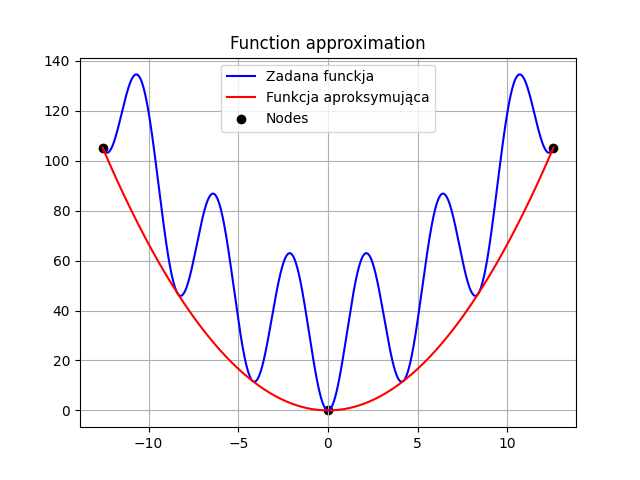
\includegraphics[width=\textwidth]{img01.png}
    \caption{Wykres dla 12 równoodległych węzłów}
  \end{minipage}
  \hfill
  \begin{minipage}[b]{0.49\textwidth}
    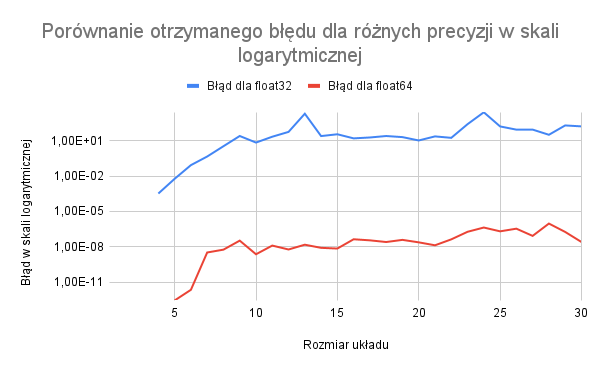
\includegraphics[width=\textwidth]{img02.png}
    \caption{Wykres dla 12 węzłów Czebyszewa}
  \end{minipage}
\end{figure}

\subsubsection{Efekt Rungego}

Efekt Rungego występuje jedynie dla nie węzłów równoodległych, jak widać na poniższym wykresie.

\begin{figure}[H]
\centering
  \begin{minipage}[b]{0.49\textwidth}
    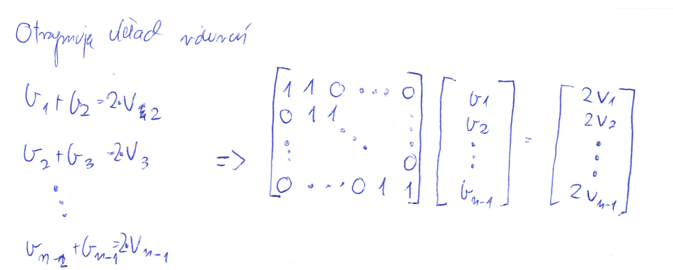
\includegraphics[width=\textwidth]{img07.png}
    \caption{Efekt Rungego dla 15 równoodległych węzłów}
  \end{minipage}
\end{figure}

\subsubsection{Najlepsze przybliżenie}

Najlepsze przybliżenie ze względu na błąd maksymalny (dla 50 węzłów) oraz średniokwadratowy (dla 54 węzłów), można otrzymać korzystając jedynie z generacji węzłów zgodnie z zerami wielomianu Czebyszewa, a wartości błędów są dużo mniejsze niż w przypadku węzłów równoodległych.

\begin{figure}[H]
  \begin{minipage}[b]{0.49\textwidth}
    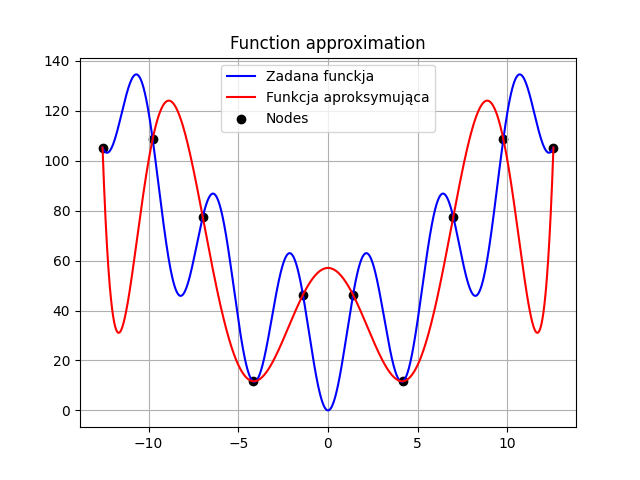
\includegraphics[width=\textwidth]{img05.png}
    \caption{Najlepsze przybliżenie ze względu na błąd maksymalny}
  \end{minipage}
  \hfill
  \begin{minipage}[b]{0.49\textwidth}
    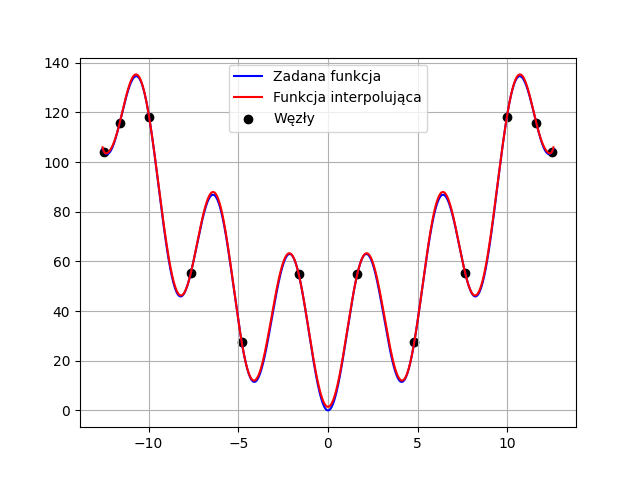
\includegraphics[width=\textwidth]{img06.png}
    \caption{Najlepsze przybliżenie ze względu na błąd średniokwadratowy}
  \end{minipage}
\end{figure}

Na poniższych wykresach są podane wartości błędów dla powyższych wykresów.

\begin{table}[!ht]
    \centering
    \begin{tabular}{|l|l|}
    \hline
        Błąd maksymalny & 1.9895196601282805e-13 \\ \hline
        Błąd średniokwadratowy & 2.296897441475515e-27 \\ \hline
    \end{tabular}
    \caption{Wartości błędów}
\end{table}

\subsubsection{Spostrzeżenia}

\begin{itemize}
    \item W przypadku interpolowanej funkcji algorytm Lagrange'a wraz z węzłami wyznaczonymi zgodnie z zerami wielomianu Czebyszewa okazał się dawać najlepsze rezultaty
    \item Interpolacje na równoodległych węzłach są obarczone dużym błędem ze względu na efekt Rungego
\end{itemize}

\subsection{Interpolacja Newtona}

\noindent
Poniżej na wykresie przedstawiony jest przykładowy wykres interpolacji Newtona dla różnego sposobu generacji węzłów.

\subsubsection{Przykładowe wykresy}

\begin{figure}[H]
  \begin{minipage}[b]{0.49\textwidth}
    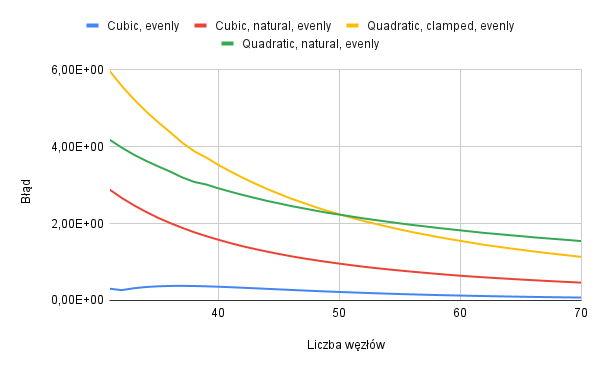
\includegraphics[width=\textwidth]{img08.png}
    \caption{Wykres dla 12 równoodległych węzłów}
  \end{minipage}
  \hfill
  \begin{minipage}[b]{0.49\textwidth}
    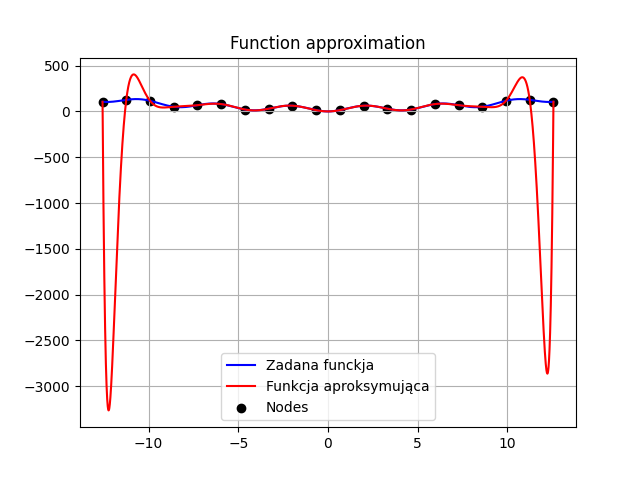
\includegraphics[width=\textwidth]{img09.png}
    \caption{Wykres dla 12 węzłów Czebyszewa}
  \end{minipage}
\end{figure}

\subsubsection{Efekt Rungego}

Efekt Rungego występuje jedynie dla nie węzłów równoodległych, jak widać na poniższym wykresie.

\begin{figure}[H]
\centering
  \begin{minipage}[b]{0.49\textwidth}
    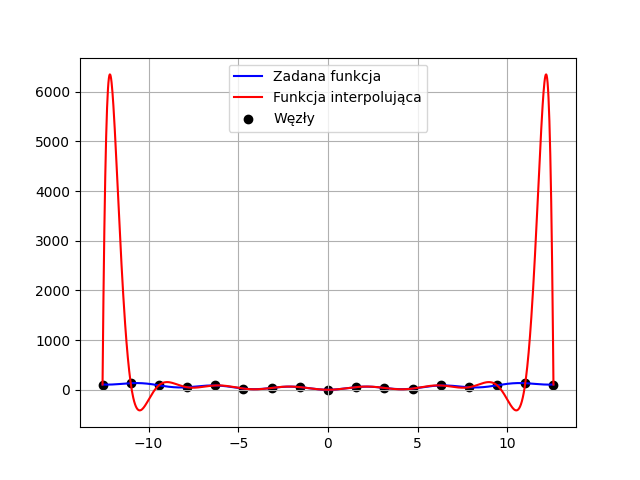
\includegraphics[width=\textwidth]{img14.png}
    \caption{Efekt Rungego dla 15 równoodległych węzłów}
  \end{minipage}
\end{figure}

\subsubsection{Najlepsze przybliżenie}

Najlepsze przybliżenie ze względu na błąd maksymalny otrzymałem dla 44 węzłów Czebyszewa oraz ze względu na błąd średniokwadratowy dla 33 równoodległych węzłów.

\begin{figure}[H]
  \begin{minipage}[b]{0.49\textwidth}
    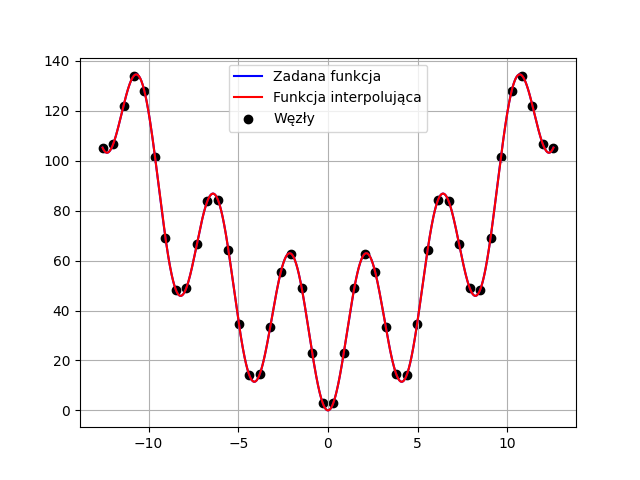
\includegraphics[width=\textwidth]{img11.png}
    \caption{Najlepsze przybliżenie ze względu na błąd maksymalny}
  \end{minipage}
  \hfill
  \begin{minipage}[b]{0.49\textwidth}
    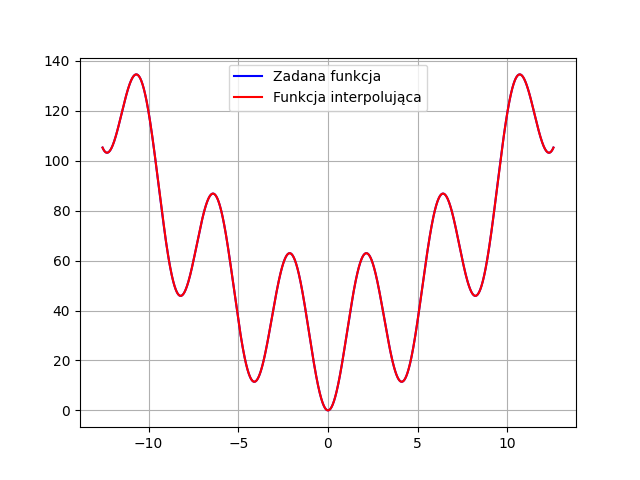
\includegraphics[width=\textwidth]{img12.png}
    \caption{Najlepsze przybliżenie ze względu na błąd średniokwadratowy}
  \end{minipage}
\end{figure}

\noindent
W poniższej tabelce podane są wartości błęów dla powyższych wykresach

\begin{table}[!ht]
    \centering
    \begin{tabular}{|l|l|}
    \hline
        Błąd maksymalny & 6.877908359115281e-05 \\ \hline
        Błąd średniokwadratowy & 8.220356191804188e-11 \\ \hline
    \end{tabular}
    \caption{Wartości błędów}
\end{table}

\subsubsection{Spostrzeżenia}

\begin{itemize}
    \item W przypadku interpolowanej funkcji algorytm Newtona wraz z węzłami wyznaczonymi zgodnie z zerami wielomianu Czebyszewa okazał się dawać najlepsze rezultaty
    \item Interpolacje na równoodległych węzłach są obarczone dużym błędem ze względu na efekt Rungego
    \item Algorytm Newtona przy dużej ilości węzłów zaczyna generować ogromne błędy z uwagi na niedokładną reprezentacje liczb zmiennoprzecinkowych
\end{itemize}

\subsection{Interpolacja Hermite'a}

\noindent
Poniżej na wykresie przedstawiony jest przykładowy wykres interpolacji Hermite'a dla różnego sposobu generacji węzłów.

\subsubsection{Przykładowe wykresy}

\begin{figure}[H]
  \begin{minipage}[b]{0.49\textwidth}
    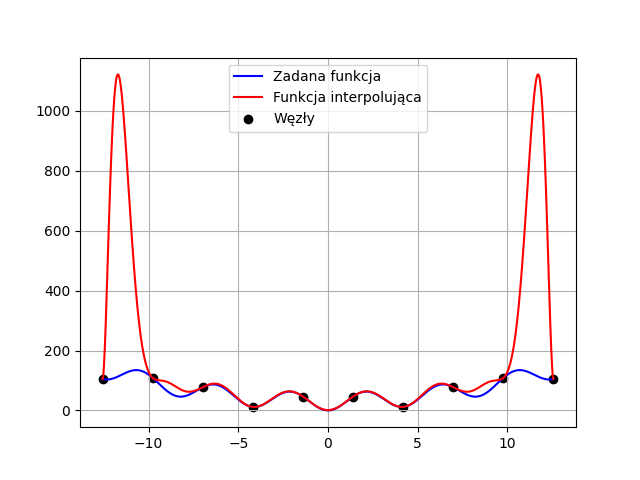
\includegraphics[width=\textwidth]{img15.png}
    \caption{Wykres dla 12 równoodległych węzłów}
  \end{minipage}
  \hfill
  \begin{minipage}[b]{0.49\textwidth}
    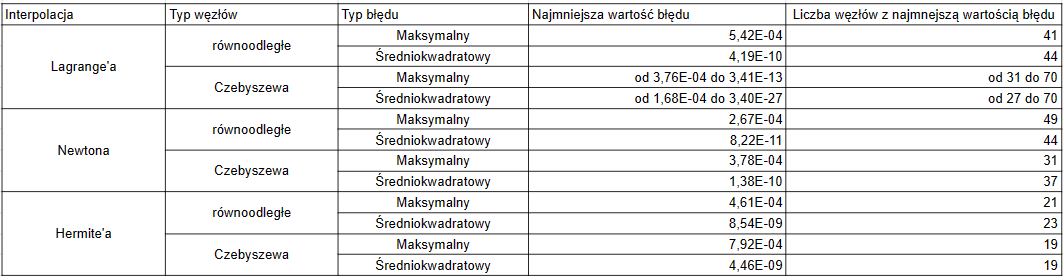
\includegraphics[width=\textwidth]{img16.png}
    \caption{Wykres dla 12 węzłów Czebyszewa}
  \end{minipage}
\end{figure}

\subsubsection{Efekt Rungego}

Efekt Rungego występuje jedynie dla nie węzłów równoodległych, jak widać na poniższym wykresie.

\begin{figure}[H]
\centering
  \begin{minipage}[b]{0.49\textwidth}
    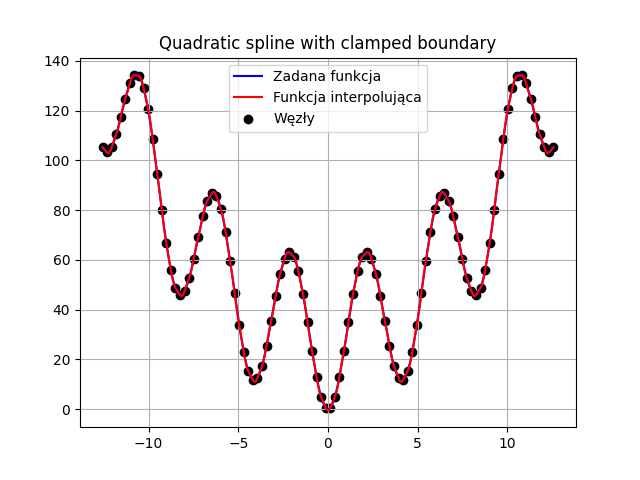
\includegraphics[width=\textwidth]{img21.png}
    \caption{Efekt Rungego dla 12 równoodległych węzłów}
  \end{minipage}
\end{figure}

\subsubsection{Najlepsze przyblizenie}

Najlepsze przybliżenie ze względu na błąd maksymalny otrzymałem dla 17 węzłów Czebyszewa oraz ze względu na błąd średniokwadratowy również dla 17 węzłów Czebyszewa.

\begin{figure}[H]
  \begin{minipage}[b]{0.49\textwidth}
    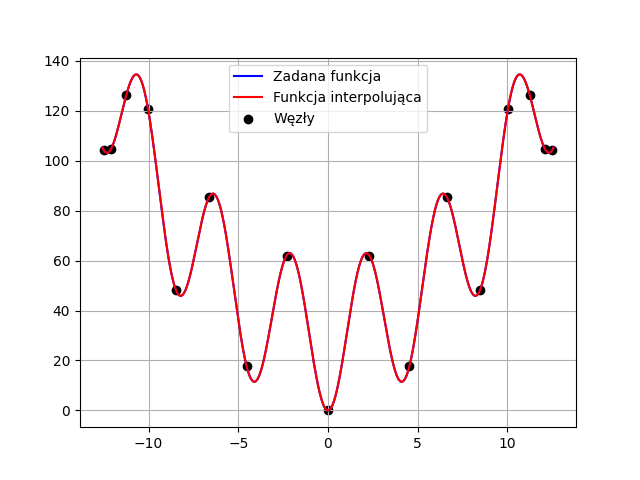
\includegraphics[width=\textwidth]{img19.png}
    \caption{Najlepsze przybliżenie ze względu na błąd maksymalny}
  \end{minipage}
  \hfill
  \begin{minipage}[b]{0.49\textwidth}
    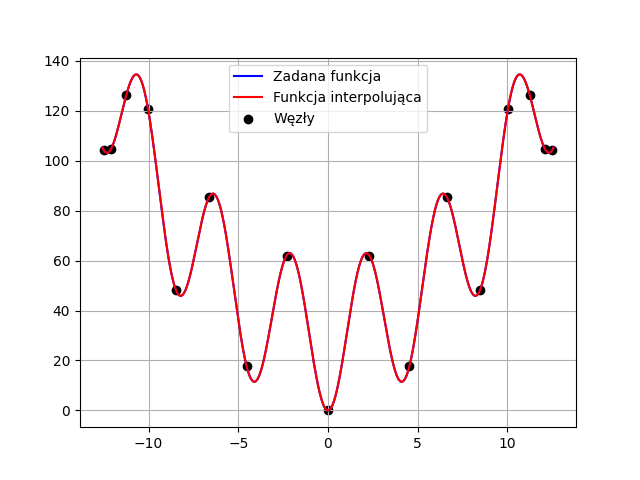
\includegraphics[width=\textwidth]{img20.png}
    \caption{Najlepsze przybliżenie ze względu na błąd średniokwadratowy}
  \end{minipage}
\end{figure}

\noindent
W poniższej tabelce podane są wartości błęów dla powyższych wykresów

\begin{table}[!ht]
    \centering
    \begin{tabular}{|l|l|}
    \hline
        Błąd maksymalny & 0.0002819640489661879 \\ \hline
        Błąd średniokwadratowy & 1.1739707228164544e-09 \\ \hline
    \end{tabular}
    \caption{Wartości błędów}
\end{table}

\subsubsection{Spostrzeżenia}

\begin{itemize}
\item Dla małej ilości węzłów (do 20) lepsze przybliżenie funkcji dają węzły Czebyszewa
\item Błąd maksymalny pozwala trafnie określić, gdzie zachodzi efekt Rungego (dla małej ilości węzłów). Dla dużej ilości węzłów bardzo widoczny jest problem z reprezentacją liczb zmiennoprzecinkowych w komputerze, ponieważ otrzmane wartości błędów są ogromne
\item Iterpolacja Hermite'a daje dobre przybliżenie dla odpowiednio dobranej liczby węzłów.
\end{itemize}

\subsection{Interpolacja funkcją sklejaną 2-go stopnia}

\subsubsection{Przykładowe wykresy}

\noindent
Poniżej znajdują się przykładowe wykresy prezentujące interpolację przy pomocy funkcji sklejanej 2-go stopnia. Jeden dla natural boundary, a drugi dla clamped boundary

\begin{figure}[H]
  \begin{minipage}[b]{0.49\textwidth}
    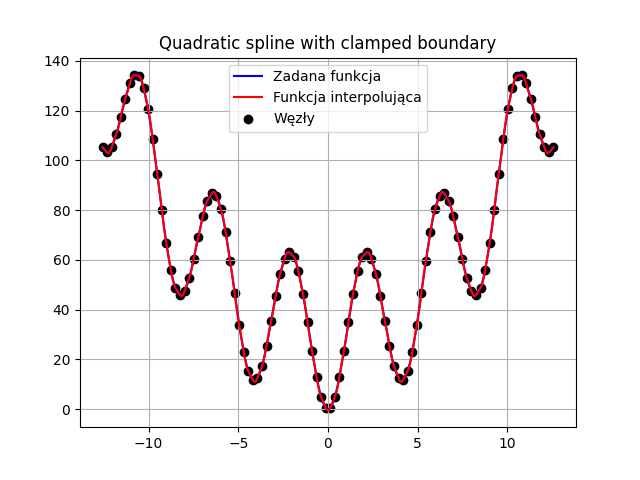
\includegraphics[width=\textwidth]{img22.png}
    \caption{Wykres dla 12 węzłów i natural boundary}
  \end{minipage}
  \hfill
  \begin{minipage}[b]{0.49\textwidth}
    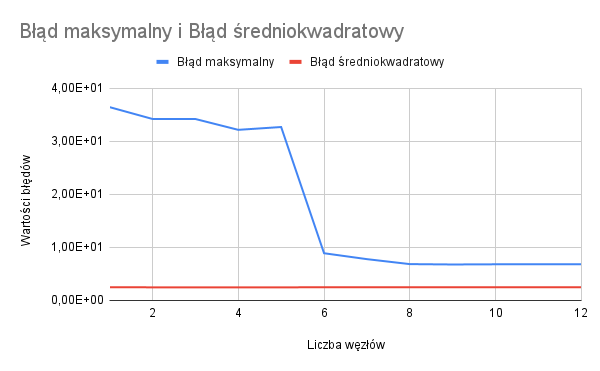
\includegraphics[width=\textwidth]{img23.png}
    \caption{Wykres dla 12 węzłów  i clamped boundary}
  \end{minipage}
\end{figure}

\subsubsection{Najlepsze przyblizenie}

Najlepsze przybliżenie ze względu na błąd maksymalny jak i średniokwadratowy otrzymałem dla clamped boundary i 100 węzłów.

\begin{figure}[H]
  \begin{minipage}[b]{0.49\textwidth}
    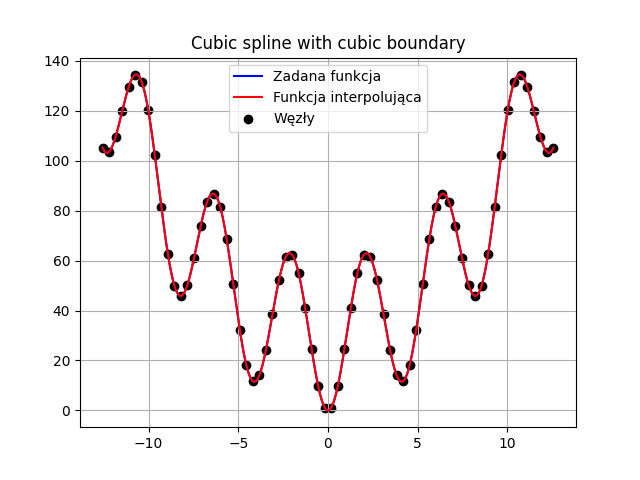
\includegraphics[width=\textwidth]{img26.png}
    \caption{Najlepsze przybliżenie ze względu na błąd maksymalny}
  \end{minipage}
  \hfill
  \begin{minipage}[b]{0.49\textwidth}
    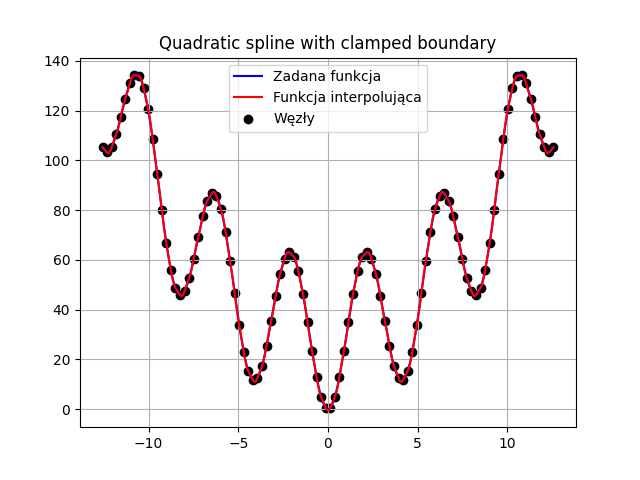
\includegraphics[width=\textwidth]{img27.png}
    \caption{Najlepsze przybliżenie ze względu na błąd średniokwadratowy}
  \end{minipage}
\end{figure}

\noindent
W poniższej tabelce podane są wartości błęów dla powyższych wykresów

\begin{table}[!ht]
    \centering
    \begin{tabular}{|l|l|}
    \hline
        Błąd maksymalny & 0.5527769402251668 \\ \hline
        Błąd średniokwadratowy & 0.16001239042418153 \\ \hline
    \end{tabular}
    \caption{Wartości błędów}
\end{table}

\subsection{Interpolacja funkcją sklejaną 3-go stopnia}

\subsubsection{Przykładowe wykresy}

\noindent
Poniżej znajdują się przykładowe wykresy reprezentujące działanie funkcji sklejanej 3-go stopnia dla 2 różnych warunków - default boundary i natural boundary.

\begin{figure}[H]
  \begin{minipage}[b]{0.49\textwidth}
    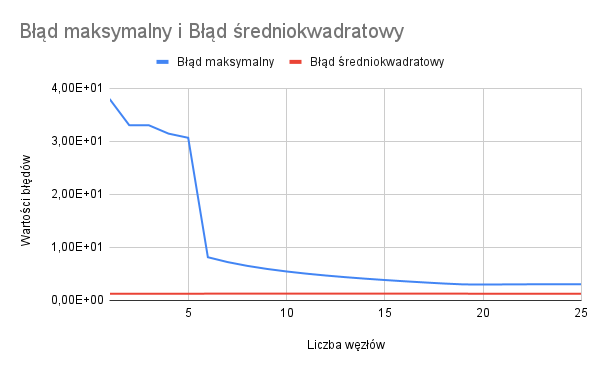
\includegraphics[width=\textwidth]{img28.png}
    \caption{Wykres dla 12 węzłów i default boundary}
  \end{minipage}
  \hfill
  \begin{minipage}[b]{0.49\textwidth}
    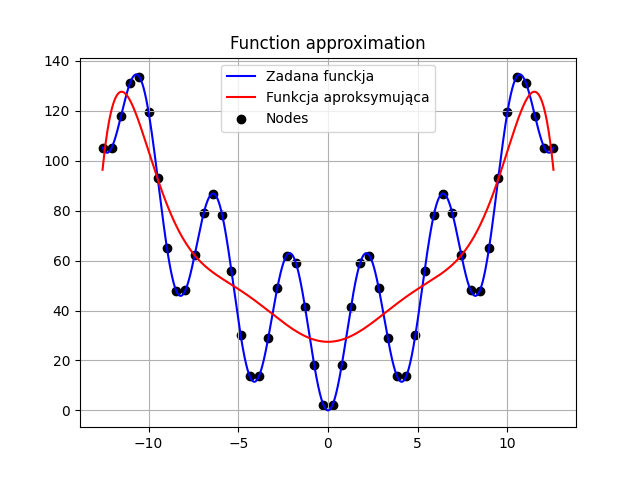
\includegraphics[width=\textwidth]{img29.png}
    \caption{Wykres dla 12 węzłów i clamped boundary}
  \end{minipage}
\end{figure}

\subsubsection{Najlepsze przyblizenie}

Najlepsze przybliżenie, ze względu na błąd maskymalny otzymałem dla default boundary i 100 węzłów, a ze względu na błąd średniokwadratowy dla natural boundary i również 100 węzłów.

\begin{figure}[H]
  \begin{minipage}[b]{0.49\textwidth}
    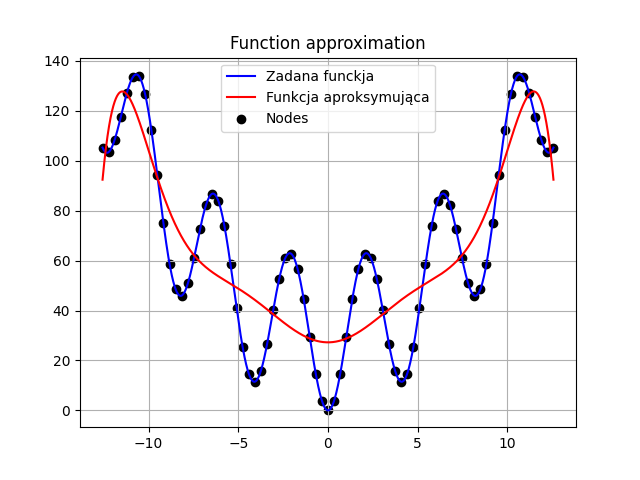
\includegraphics[width=\textwidth]{img30.png}
    \caption{Najlepsze przybliżenie ze względu na błąd maksymalny}
  \end{minipage}
  \hfill
  \begin{minipage}[b]{0.49\textwidth}
    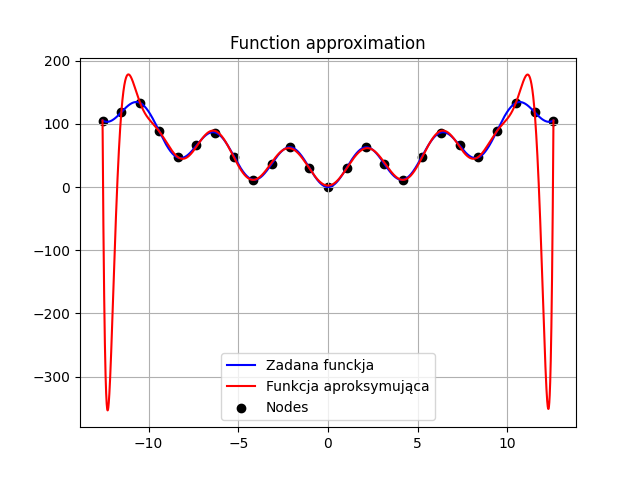
\includegraphics[width=\textwidth]{img33.png}
    \caption{Najlepsze przybliżenie ze względu na błąd średniokwadratowy}
  \end{minipage}
\end{figure}

\noindent
W poniższej tabelce podane są wartości błęów dla powyższych wykresów

\begin{table}[!ht]
    \centering
    \begin{tabular}{|l|l|}
    \hline
        Błąd maksymalny & 0.020287863798969852 \\ \hline
        Błąd średniokwadratowy & 0.0005181051145680916 \\ \hline
    \end{tabular}
    \caption{Wartości błędów}
\end{table}

\subsection{Aproksymacja średniokwadratowa wielomianem algebraicznym}

\subsubsection{Przykładowe wykresy}

\noindent


\begin{figure}[H]
  \begin{minipage}[b]{0.49\textwidth}
    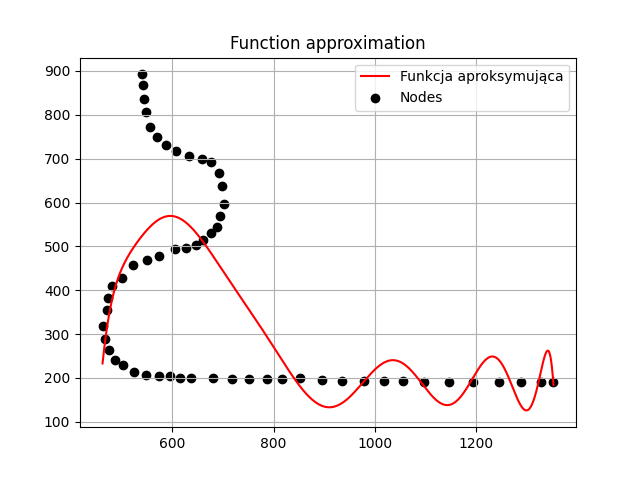
\includegraphics[width=\textwidth]{img.png}
    \caption{Wykres dla }
  \end{minipage}
  \hfill
  \begin{minipage}[b]{0.49\textwidth}
    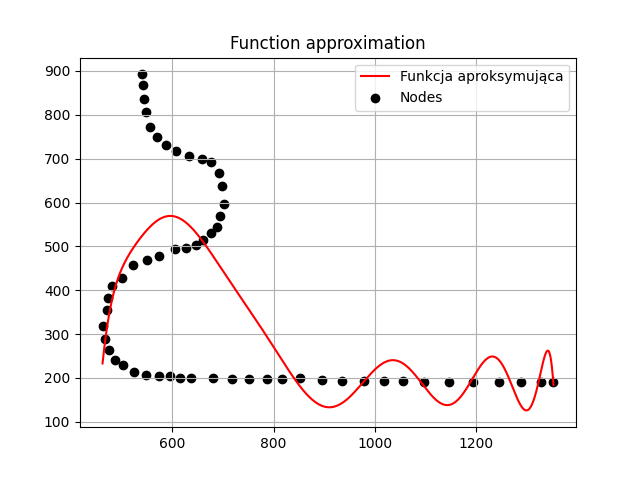
\includegraphics[width=\textwidth]{img.png}
    \caption{Wykres dla }
  \end{minipage}
\end{figure}

\subsubsection{Najlepsze przyblizenie}


\begin{figure}[H]
  \begin{minipage}[b]{0.49\textwidth}
    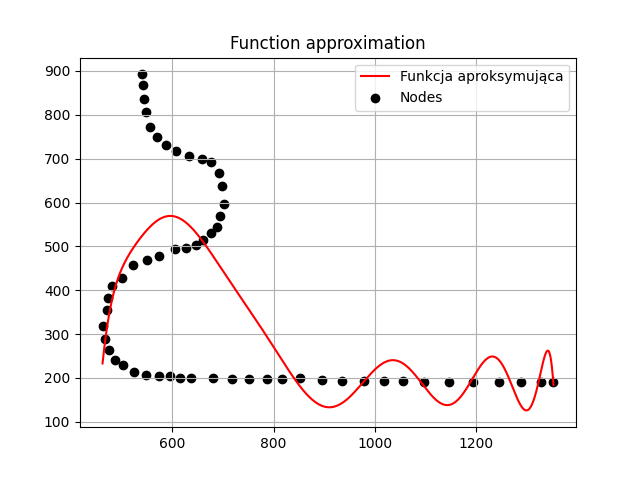
\includegraphics[width=\textwidth]{img.png}
    \caption{Najlepsze przybliżenie ze względu na błąd maksymalny}
  \end{minipage}
  \hfill
  \begin{minipage}[b]{0.49\textwidth}
    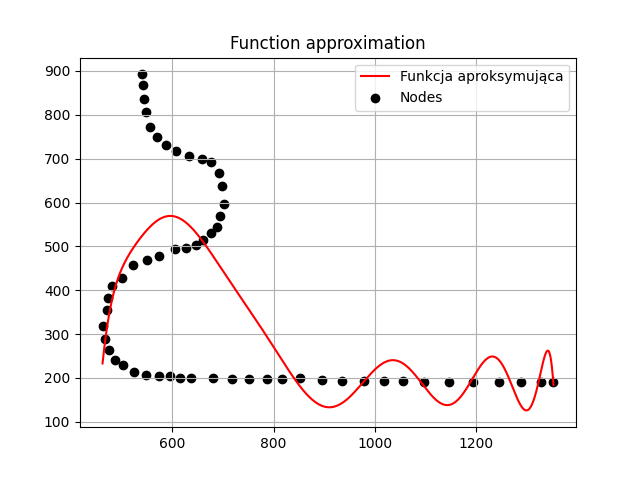
\includegraphics[width=\textwidth]{img.png}
    \caption{Najlepsze przybliżenie ze względu na błąd średniokwadratowy}
  \end{minipage}
\end{figure}

\noindent
W poniższej tabelce podane są wartości błęów dla powyższych wykresów





\end{document}
